\item \textbf{{[}ALVL/9597/2017/P1/Q3{]} }

A data structure is required to store 25 nodes. A linked list is maintained
of all the nodes. A node contains a data value and two pointers: a
left pointer and a right pointer. 

Items in the list are initially linked using their \texttt{LeftChild}
pointers. 

Each node ls implemented as an instance of the class \texttt{ConnectionNode}.
The class ConnectionNode has the following properties: 
\begin{center}
\begin{tabular}{|l|l|l|}
\hline 
\multicolumn{3}{|c|}{\texttt{Class: Connection Node}}\tabularnewline
\hline 
\multicolumn{3}{|c|}{Attributes}\tabularnewline
\hline 
\texttt{\hspace{0.01\columnwidth}}Identifier & \texttt{\hspace{0.01\columnwidth}}Data Type & \texttt{\hspace{0.05\columnwidth}}Description\tabularnewline
\hline 
\texttt{DataValue} & \texttt{STRING} & The node data\tabularnewline
\hline 
\texttt{LeftChild} & \texttt{INTEGER} & The left node pointer \tabularnewline
\hline 
\texttt{RightChild} & \texttt{INTEGER} & The right node pointer\tabularnewline
\hline 
\end{tabular}
\par\end{center}

The structure for the linked list is implemented as follows: 
\begin{center}
\begin{tabular}{|l|c|l|}
\hline 
\texttt{\hspace{0.01\columnwidth}}Identifier & Data Type & \texttt{\hspace{0.05\columnwidth}}Description\tabularnewline
\hline 
\texttt{RobotData} & \texttt{ARRAY {[}l : 25{]} OF ConnectionNode} & An array used to store the\tabularnewline
 &  & 25 nodes.\tabularnewline
\hline 
\texttt{Root} & \texttt{INTEGER} & Index for the root position \tabularnewline
 &  & of the \texttt{RobotData} array\tabularnewline
\hline 
\texttt{NextFreeChild} & \texttt{INTEGER} & Index for the next \tabularnewline
 &  & available empty node\tabularnewline
\hline 
\end{tabular}
\par\end{center}

The first available node Is indicated by \texttt{NextFreeChild}. The
initial value of \texttt{Root} is 1 and the initial value of \texttt{NextFreeChild}
is 1.

The diagram shows the empty data structure with the linked list to
record the unused nodes. 
\begin{center}
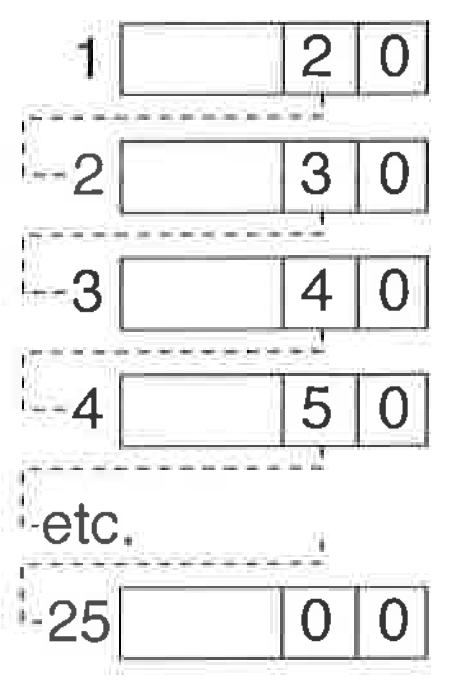
\includegraphics[width=0.125\paperwidth]{C:/Users/Admin/Desktop/Github/question_bank/LyX/static/img/9597-ALVL-2017-P1-Q3-1}
\par\end{center}

\subsubsection*{Task 3.1}

Write the program code to declare the \textbf{empty} data structure
and linked list of 25 unused nodes. Add statement(s) to initiallse
the empty data structure.

\subsubsection*{Evidence 6}

Your program code for Task 3.1. \hfill{}{[}12{]}

This data structure is used to record the possible routes for a robot
to travel from a node A to a node Z. The following data structure
illustrates many possible routes, for example, A$\rightarrow$D$\rightarrow$K$\rightarrow$L$\rightarrow$M$\rightarrow$Z.
It is only possible to move to one of two possible nodes; for example,
from node A, the only move is to node B or node D.
\begin{center}
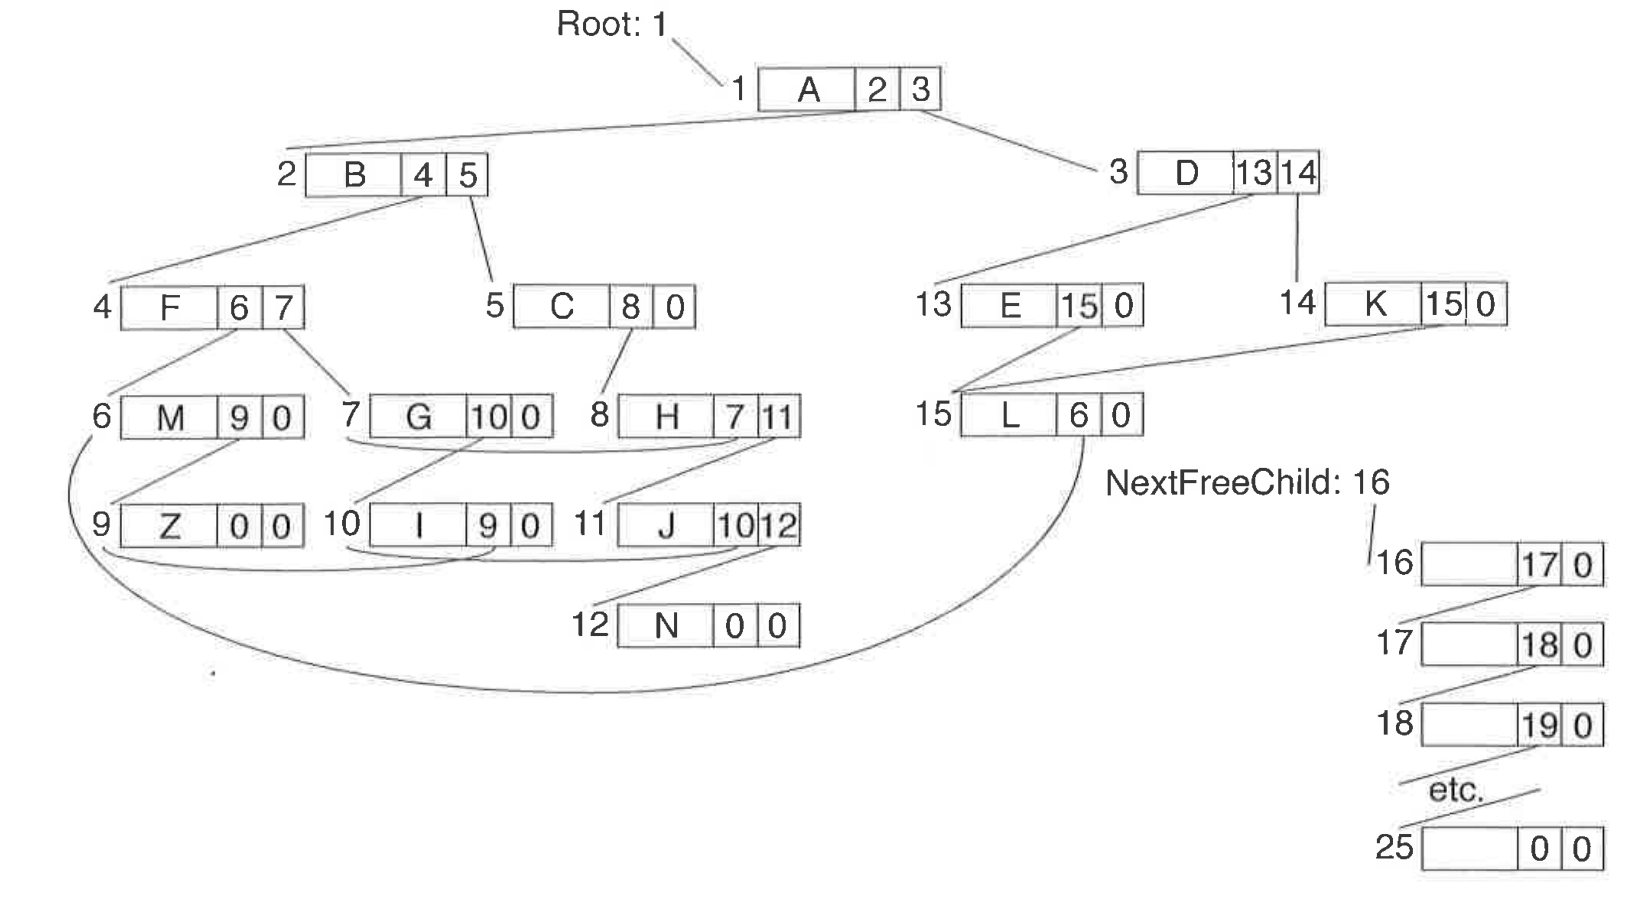
\includegraphics[width=0.5\paperwidth]{C:/Users/Admin/Desktop/Github/question_bank/LyX/static/img/9597-ALVL-2017-P1-Q3-2}
\par\end{center}

This data structure has 15 nodes (A to N and Z) but for future development
a maximum of 25 nodes is specified. All nodes are unique.

The pseudocode on the next page can be used to add a node to the data
structure. The procedure \texttt{AddToRobotData} uses the parameters
\texttt{NewDataItem}, \texttt{ParentItem} and \texttt{ThisMove}.

The parameter \texttt{ThisMove} holds the move made to create this
new item (\textquoteleft L' for LeftChild, \textquoteleft R' for RightChild,
\textquoteleft X\textquoteright{} for initial state/root), and the
\texttt{ParentItem} parameter holds the value of the parent item which
points to this \texttt{NewDataItem}.
\begin{center}
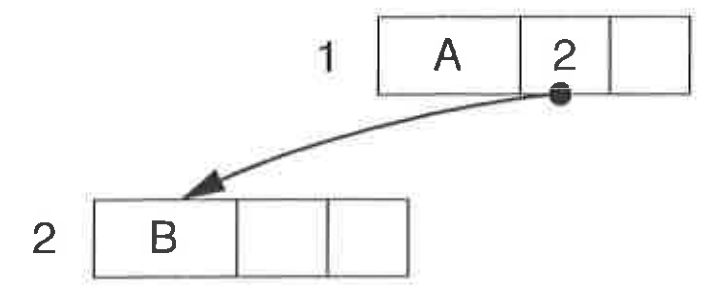
\includegraphics[width=0.25\paperwidth]{C:/Users/Admin/Desktop/Github/question_bank/LyX/static/img/9597-ALVL-2017-P1-Q3-3}
\par\end{center}

To add node B as shown, the procedure call would be \texttt{AddToRobotData
('B', \textquoteleft A', 'L')} . The parameters used would be: 

\texttt{B}, the new node 

\texttt{A}, the parent node 

\texttt{L}, the location of the child (which has an index of 2) is
recorded in \texttt{LeftChild} of A.

The following pseudocode (available in PS EUDOCODE\_TASK\_3\_2 . TXT)
can be used to add a node to the data structure.

\noindent %
\noindent\begin{minipage}[t]{1\columnwidth}%
\texttt{FUNCTION FindNode(NodeValue) RETURNS INTEGER }

\texttt{\qquad{}Found <- FALSE}

\texttt{\qquad{}CurrentPosition <- Root }

\texttt{\qquad{}REPEAT }

\texttt{\qquad{}\qquad{}IF RobotData{[}CurrentPosition{]}.DataValue
= NodeValue THEN }

\texttt{\qquad{}\qquad{}\qquad{}Found <- TRUE }

\texttt{\qquad{}\qquad{}ELSE }

\texttt{\qquad{}\qquad{}\qquad{}CurrentPosition <- CurrentPosition
+ 1 }

\texttt{\qquad{}\qquad{}ENDIF }

\texttt{\qquad{}UNTIL Found = TRUE OR CurrentPosition > 25 }

\texttt{\qquad{}IF CurrentPOSition > 25 THEN }

\texttt{\qquad{}\qquad{}RETURN 0}

\texttt{\qquad{}ELSE }

\texttt{\qquad{}\qquad{}RETURN CurrentPosition }

\texttt{\qquad{}ENDIF }

\texttt{ENDFUNCTION}

\bigskip{}

\texttt{PROCEDURE AddToRobotData(NewDataItem, ParentItem, ThisMove) }

\texttt{\qquad{}\qquad{}IF Root = 1 AND NextFreeChild = 1 THEN }

\texttt{\qquad{}\qquad{}\qquad{}NextFreeChild <- RobocData{[}NextFreeChild{]}.LeftChild }

\texttt{\qquad{}\qquad{}\qquad{}RobotDataIRoot{]}.LeftChild <-
0 }

\texttt{\qquad{}\qquad{}\qquad{}RobotData{[}Root{]}.DataValue <-
NewDataItem }

\texttt{\qquad{}\qquad{}ELSE }

\texttt{\qquad{}\qquad{}\qquad{}// does the parent exist? . }

\texttt{\qquad{}\qquad{}\qquad{}ParentPosition <- FindNode(ParentItem) }

\texttt{\qquad{}\qquad{}\qquad{}IF RarentPosition > 0 THEN // parent
exists }

\texttt{\qquad{}\qquad{}\qquad{}\qquad{}// does the child exist? }

\texttt{\qquad{}\qquad{}\qquad{}\qquad{}ExistingChild <- FindNode(NewDataItem)
' }

\texttt{\qquad{}\qquad{}\qquad{}\qquad{}IF ExistingChild > 0 THEN
// child exists }

\texttt{\qquad{}\qquad{}\qquad{}\qquad{}\qquad{}ChildPointer
<- ExistingChild }

\texttt{\qquad{}\qquad{}\qquad{}\qquad{}ELSE }

\texttt{\qquad{}\qquad{}\qquad{}\qquad{}ChildPointer <- NextFreeChild }

\texttt{\qquad{}\qquad{}\qquad{}\qquad{}NextFreeChild <- RobotDataINextFreeChild\}.LeftChild }

\texttt{\qquad{}\qquad{}\qquad{}\qquad{}RobotData{[}ChildPointer{]}.LeftChild
<- 0 }

\texttt{\qquad{}\qquad{}\qquad{}\qquad{}RobotData{[}ChildPointer{]}.DataValue
<- NewDataItem }

\texttt{\qquad{}\qquad{}\qquad{}\qquad{}ENDIF }

\texttt{\qquad{}\qquad{}\qquad{}\qquad{}IF ThisMove = 'L' THEN }

\texttt{\qquad{}\qquad{}\qquad{}\qquad{}\qquad{}RobotData{[}ParentPosition{]}.LeftChild
<- ChildPointer }

\texttt{\qquad{}\qquad{}\qquad{}\qquad{}ELSE }

\texttt{\qquad{}\qquad{}\qquad{}\qquad{}\qquad{}RobotData{[}ParentPosition{]}.RightChild
<- ChildPointer }

\texttt{\qquad{}\qquad{}\qquad{}\qquad{}ENDIF }

\texttt{\qquad{}\qquad{}\qquad{}ENDIF}\textbf{ }

\texttt{\qquad{}\qquad{}ENDIF }

\texttt{ENDPROCEDURE}%
\end{minipage}

\subsubsection*{Task 3.2}

Write code to implement \texttt{AddToRobotData} and \texttt{FindNode}
from this pseudocode.

You may use the text file \texttt{PSEUDOCODE\_TASK\_3\_2.TXT} as a
basis for writing your code.

\subsubsection*{Evidence 7}

Your program code for Task 3.2. \hfill{}{[}7{]}

\subsubsection*{Task 3.3}

Write a procedure \texttt{OutputData} which displays the value of
\texttt{Root}, the value of \texttt{NextFreeChild} and the contents
of \texttt{RobotData} in index order.

\subsubsection*{Evidence 8}

Your program code for Task 3.3.\hfill{} {[}6{]}

\subsubsection*{Task 3.4}

The file \texttt{SEARCHTREE.TXT} contains the data for the search
tree. Each row of the file contains three comma separated values,
for example, the first row contains '\texttt{A}', '\texttt{0}' and
'X'. The file is organised as: \texttt{NewDataltem, ParentItem, ThisMove}

\texttt{NewDataItem, ParentItem, ThisMove}

\texttt{$\dots$}

\texttt{<End of File>}

There are a total of 20 lines in the \texttt{SEARCHTREE.TXT} file
representing possible routes.

Write a main program to read the contents of this file and use \texttt{AddToRobotData}
and \texttt{FindNode} to insert these routes into \texttt{RobotData}.
Your program will then call the \texttt{OutputData} procedure. 

\subsubsection*{Evidence 9}

Your program code for Task 3.4. \hfill{}{[}6{]}

\subsubsection*{Evidence 10}

Screenshot showing the output from running the program in Task 3.4.\hfill{}
{[}2{]}

\subsubsection*{Task 3.5}

Write a recursive pre-order tree traversal that will display all valid
routes from A to Z by following the routes described in \texttt{RobotData}.

\subsubsection*{Evidence 11}

Your program code for Task 3.5.\hfill{} {[}6{]}

\subsubsection*{Evidence 12}

Screenshot showing the output from running the program in Task 3.5.\hfill{}
{[}1{]}